% la-08-bayes.tex

\documentclass[xcolor=dvipsnames]{beamer}
\usepackage{tikz}
\usepackage{teachbeamer}

\title{Axioms and Theorems of Probability}
\subtitle{{\CourseNumber}, BCIT}

\author{\CourseName}

\date{November 13, 2018}

\begin{document}

\begin{frame}
  \titlepage
\end{frame}

\begin{frame}
  \frametitle{Introductory Concepts in Statistics I}
  \begin{itemize}
  \item<1-> A \alert{population} is the complete collection of all
    measurements or data that are being considered.
  \item<2-> A \alert{census} is the collection of data from every
    member of the population.
  \item<3-> A \alert{sample} is a subcollection of members selected
    from a population.
  \end{itemize}
\end{frame}

\begin{frame}
  \frametitle{Introductory Concepts in Statistics II}
  \begin{itemize}
  \item<1-> A \alert{voluntary response sample} or
    \alert{self-selected sample} is one in which the respondents
    themselves decide whether to be included.
  \item<2-> A \alert{random sample} is one in which each member has
    the same probability of being selected.
  \item<3-> A \alert{stratified random sample} is one in which random
    samples from subgroups are drawn and proportionally combined to
    form the complete sample.
  \end{itemize}
\end{frame}

\begin{frame}
  \frametitle{Introductory Concepts in Statistics III}
  \begin{itemize}
  \item<1-> A \alert{parameter} is a numerical measurement describing
    some characteristic of the population.
  \item<2-> A \alert{statistic} is a numerical measurement describing
    some characteristic of a sample.
  \end{itemize}
\end{frame}

\begin{frame}
  \frametitle{Introductory Concepts in Statistics IV}
  \begin{itemize}
  \item<1-> \alert{Quantitative} (or \alert{numerical}) data consist
    of numbers representing counts or measurements.
  \item<2-> \alert{Categorical} (or \alert{qualitative}) data consist
    of names or labels that are not numbers representing counts or
    measurements.
  \end{itemize}
\end{frame}

\begin{frame}
  \frametitle{Introductory Concepts in Statistics V}
  \begin{itemize}
  \item<1-> \alert{Discrete} data result when the data values are
    quantitative and the number of values is finite or countable.
  \item<2-> \alert{Continuous} data result when the data values are
    quantitative and the number of values is infinite and not
    countable.
  \end{itemize}
Here is an example for infinite discrete outcomes (this is rare). Roll
a die until you roll a six. There are infinitely many ways to do this,
but the data is not continuous.
\end{frame}

\begin{frame}
  \frametitle{Introductory Concepts in Statistics VI}
  \begin{itemize}
  \item<1-> \alert{Blinding} is when the subject doesn't know whether
    they are receiving a treatment or a placebo.
  \item<2-> The \alert{placebo effect} occurs when an untreated
    subject reports an improvement in symptoms because of their
    participation in the study.
  \item<3-> An experiment is \alert{double-blind} when it is blind and
    the experimenter also doesn't know whether they are applying a
    treatment or a placebo.
  \end{itemize}
\end{frame}

\begin{frame}
  \frametitle{Correlation Does Not Imply Causation}
\alert{Confounding} occurs in an experiment when the investigators are
not abloe to distinguish among the effects of different factors.
\begin{figure}[h]
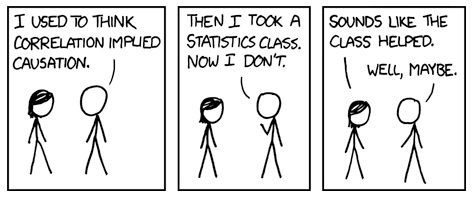
\includegraphics[scale=.3]{./diagrams/xkcd-causation-correlation.png}
\end{figure}
Examples: 
\begin{enumerate}
\item<1-> astrological sign and IQ in elementary school
\item<2-> soft drinks and obesity
\item<3-> birth control pills and thrombosis
\end{enumerate}
\end{frame}

\begin{frame}
  \frametitle{Characterizing Data Sets}
  The following serve to characterize data sets without listing the
  data:
  \begin{itemize}
  \item measures of centre
  \item measures of dispersion
  \item measures of position
  \end{itemize}
\end{frame}

\begin{frame}
  \frametitle{Measures of Centre: Mean}
  \begin{equation}
    \label{eq:daechuev}
    \mbox{mean}=\frac{\sum{}x}{n}
  \end{equation}
  where $n$ is the number of data points in your quantitative data set
  and $x$ is your data set. Mathematically speaking, $x$ is an
  $n$-dimensional vector $x=(x_{1},{\ldots},x_{n})$ and $\sum{}x$
  means
  \begin{equation}
    \label{eq:aethecux}
    \sum{}x=x_{1}+{\ldots}x_{n}
  \end{equation}
Often, we write $\mu$ for the mean of a
  population and $\bar{x}$ for the mean of a sample.
\end{frame}

\begin{frame}
  \frametitle{Frequency Distributions}
Often, data is provided in the form of a frequency distribution. For
example, when I asked a class of statistics students about the number
of countries they had visited in their lifetime, the response was as
follows (given as an R command),
\begin{alltt}
\small
cn<-c(5,4,7,3,6,4,3,4,2,4,4,2,4,3,2,4,4)
\end{alltt}
A more intelligible way to display the data is to provide a frequency
distribution.
\begin{alltt}
> table(cn)\newline
cn\newline
2 3 4 5 6 7 \newline
3 3 8 1 1 1
\end{alltt}
There are 3 people who have been to 2 countries, 3 people who have
been to 3 countries, 8 people who have been to 4 countries, 1 person
who has been to 5 countries, and so on.
\end{frame}

\begin{frame}
  \frametitle{Calculating the Mean from a Frequency Distribution}
If you have a frequency distribution (usually of a sample, so we will
call the mean $\bar{x}$), the mean is 
\begin{equation}
  \label{eq:eogheivi}
  \bar{x}=\frac{\sum{}\left(f\cdot{}x\right)}{\sum{}f}
\end{equation}
For the example in the last slide,
\begin{equation}
  \label{eq:uevuemoo}
  \bar{x}=\frac{2\cdot{}3+3\cdot{}3+4\cdot{}8+5\cdot{}1+6\cdot{}1+7\cdot{}1}{3+3+8+1+1+1}\approx{}3.82
\end{equation}
In R, you can also simply use the command \texttt{mean}. Notice that
\texttt{mean(x)} and \texttt{sum(x)/length(x)} will give you the same
number.
\end{frame}

\begin{frame}
  \frametitle{Exercises}
  {\ubung} Find the mean of the following five counts for Chips Ahoy
  chocolate chip cookies: 22 chips, 22, chips, 26 chips, 24 chips, and
  23 chips.

  \bigskip

  {\ubung} Anne measures the temperature in her walk-in freezer. She
  measures $-23^{\circ}$C once; $-22^{\circ}$C 31 times;
  $-21^{\circ}$C 13 times; $-20^{\circ}$C 7 times; $-18^{\circ}$C
  twice. What is the mean temperature given this dataset?
\end{frame}

\begin{frame}
  \frametitle{Measures of Centre: Median}
The median is the value in the middle. If there is an even number of
data points, the median is the mean of the two data points in the
middle. To find the median, sort the data points. For example, the
numbers of countries visited are

\medskip

\begin{tabular}{|c|c|c|c|c|c|c|c|c|c|c|c|c|c|c|c|c|}\hline
2&2&2&3&3&3&4&4&\alert{4}&4&4&4&4&4&5&6&7 \\ \hline
\end{tabular}

\medskip

The value in the middle is the number 4, which is also the median of
the data. It is quite similar to the mean, which is approximately 3.82.
\end{frame}

\begin{frame}
  \frametitle{Difference Between Mean and Median}
Imagine we had one more student in the class who was a world traveler.
She had visited 112 countries! The mean is now
\begin{equation}
  \label{eq:zephahwu}
  \bar{x}=\frac{\sum{}x}{n}=\frac{177}{18}\approx{}9.83
\end{equation}
A mean of 9.83 is no longer a good summary of the data. Let's see if
the median does better.

\medskip

\begin{tabular}{|c|c|c|c|c|c|c|c|c|c|c|c|}\hline
2&2&{\ldots}&4&4&\alert{4}&\alert{4}&4&{\ldots}&6&7&112 \\ \hline
\end{tabular}

\medskip

The new median is $(4+4)/2=4$, which is a much better summary of the
data, pretty much ignoring the outlier.
\end{frame}

\begin{frame}
  \frametitle{Measures of Dispersion: Motivation}
Have a look at these two different data sets.
\begin{alltt}
x1<-c(12,12,12,12,12,12,11,12,12,13,12,12,12,12)
\end{alltt}
and
\begin{alltt}
x2<-c(15,10,14,7,17,15,11,18,12,12,15,9,7,6)
\end{alltt}
The mean of both data sets is 12. The median of both data sets is 12.
However, something about these two data sets is different. \texttt{x2}
is more dispersed than \texttt{x1}, which means that the data is
spread out more. There is more variation in \texttt{x2}. We try to
capture this variation by finding measures of dispersion.
\end{frame}

\begin{frame}
  \frametitle{Measures of Dispersion: Absolute Value of Deviation}
The difference between data points and the mean always sums to zero!
That is not helpful. If we want to make this measure of dispersion
more useful, we need to sum the \alert{absolute value of deviation}
\begin{equation}
  \label{eq:riquithu}
  \mbox{mean absolute deviation }=\frac{\sum{}\vert{}x-\bar{x}\vert}{n}
\end{equation}
For our examples \texttt{x1} and \texttt{x2}, the mean absolute
deviations are 2 and 44, respectively. Although at first glance this
measure of dispersion looks useful, it makes for very complicated
calculations that can be simplified by choosing a different way to
make all the distances between data points and mean positive: not the
absolute value, but the square of the distance.
\end{frame}

\begin{frame}
  \frametitle{Measures of Dispersion: Variance}
The \alert{variance} is calculated as follows,
\begin{equation}
  \label{eq:roongeef}
   \mbox{variance of a population }=\sigma^{2}=\frac{\sum{}(x-\mu)^{2}}{n}
\end{equation}
Something odd happens when we take the variance of a sample. If we
were to use equation (\ref{eq:roongeef}) to calculate the sample
variance for all possible samples of a population, the mean of these
sample variance would not equal the population variance. This means
that in this case the sample variance would be a \alert{biased
  estimator} of the population variance. We don't want that! To
correct for this problem and define a sample variance which is an
\alert{unbiased estimator} of the population variance, we introduce
\alert{Bessel's correction} and define
\begin{equation}
  \label{eq:ilosoama}
   \mbox{variance of a sample }=s^{2}=\frac{\sum{}(x-\bar{x})^{2}}{n-1}
\end{equation}
\end{frame}

\begin{frame}
  \frametitle{Measures of Dispersion: Standard Deviation}
One disadvantage of the variance is that it is not an intuitive
measurement of dispersion. If we take the square root of the variance,
then we get something similar to the absolute value of deviation,
which tells us approximately how far on average the data points are
from the mean. We call this measurement the \alert{standard
  deviation}
\begin{equation}
  \label{eq:boolaesh}
   \mbox{standard deviation of a population }=\sigma=\sqrt{\frac{\sum{}(x-\mu)^{2}}{n}}
\end{equation}
\begin{equation}
  \label{eq:xeiroong}
   \mbox{standard deviation of a sample }=s=\sqrt{\frac{\sum{}(x-\bar{x})^{2}}{n-1}}
\end{equation}
Why we still sometimes prefer the variance will become
clear on the next slide. The standard deviation, whether with or
without Bessel's Correction, is a biased estimator!
\end{frame}

\begin{frame}
  \frametitle{Bessel's Correction}
\begin{figure}[h]
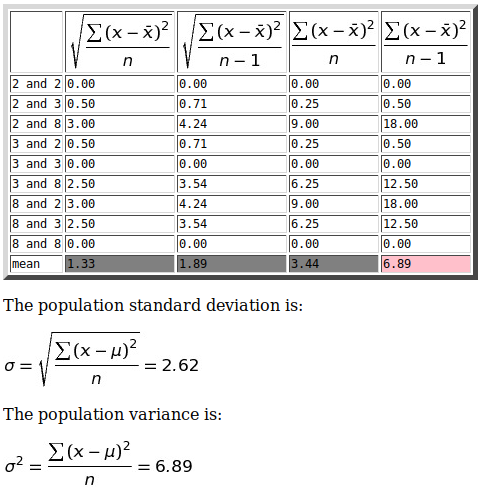
\includegraphics[scale=.45]{./diagrams/bessel.png}
\end{figure}
\end{frame}

\begin{frame}
  \frametitle{Calculating the Variance I}
It is easiest to calculate the variance using statistical software. In
R Studio, for example,
\begin{alltt}
> var(x1)\newline
[1] 0.1538462\newline
> var(x2)\newline
[1] 14.76923
\end{alltt}
and
\begin{alltt}
> sd(x1)\newline
[1] 0.3922323\newline
> sd(x2)\newline
[1] 3.843076
\end{alltt}
\end{frame}

\begin{frame}
  \frametitle{Calculating the Variance II}
When you do have to calculate the variance by hand, it is helpful to
use the following shortcut formula,
\begin{equation}
  \label{eq:eecheaxe}
s^{2}=\frac{\sum(x-\bar{x})^{2}}{n-1}=\frac{\sum{}x^{2}-\frac{\left(\sum{}x\right)^{2}}{n}}{n-1}
\end{equation}
because you do not have to keep entering the mean, which may contain
numerous significant digits.
\end{frame}

\begin{frame}
  \frametitle{Variance for a Frequency Distribution I}
Consider the data set \texttt{x3}
\begin{alltt}
4,4,2,2,4,3,3,3,1,4,4,1,2,2,2,4,2,1,2,1,1,2,3,3,2,3,3,3
\end{alltt}
We can summarize the data in a frequency distribution
\begin{alltt}
> table(x3)\newline
x3\newline
1 2 3 4 \newline
5 9 8 6 
\end{alltt}
\end{frame}

\begin{frame}
  \frametitle{Variance for a Frequency Distribution II}
Remember that in equation (\ref{eq:eogheivi}) we calculated the mean using a
formula for the frequency distribution,
\begin{equation}
  \label{eq:beingeip}
  \bar{x}=\frac{\sum{}\left(f\cdot{}x\right)}{\sum{}f}
\end{equation}
We can do the same for the variance and the standard deviation,
\begin{equation}
  \label{eq:iefoopoo}
  s^{2}=\frac{\sum{}\left(f\cdot{}x^{2}\right)-\frac{\left(\sum{}f\cdot{}x\right)^{2}}{\sum{}f}}{\sum{}f-1}
\end{equation}
Remember that $n=\sum{}f$.
\end{frame}

\begin{frame}
  \frametitle{Definitions}
  \begin{description}
  \item[event] An event is any collection of results or outcomes of a
    procedure.
  \item[sample space] The sample space for a procedure consists of all
    possible simple events. That is, the sample space consists of all
    outcomes that cannot be broken down any further. The symbol for
    the sample space is $\Omega$. 
  \item[complement] The complement of event $A$ is $\urcorner{}A$ and
    consists of all outcomes in which $A$ does not occur.
  \end{description}
\end{frame}

\begin{frame}
  \frametitle{Logic and Sets I}
  \begin{enumerate}
  \item<1-> $A\vee{}B$ is the event ``either $A$ or $B$ happens.''
  \item<2-> $A\wedge{}B$ is the event ``both $A$ and $B$ happens.''
  \item<3-> $\urcorner{}A$ is the event ``$A$ does not happens.''
  \item<4-> $\Omega$ and $\emptyset$ are events; they are called
    `tautology' and `contradiction,' respectively.
  \end{enumerate}
\end{frame}

\begin{frame}
  \frametitle{Logic and Sets II}
  The logical statement $A\vee{}B$ corresponds to the union of sets
  $A\cup{}B$ if $A$ and $B$ are understood as sets of simple events.

\medskip

  The logical statement $A\wedge{}B$ corresponds to the intersection of sets
  $A\cap{}B$ if $A$ and $B$ are understood as sets of simple events.

\medskip

Events $A$ and $B$ are \alert{disjoint} (or \alert{mutually
  exclusive}) if they cannot occur together. In set theory, we can
express this by saying that they are disjoint if and only if
$A\cap{}B=\emptyset$.

Think of dice rolls as an example. $\Omega=\{1,2,3,4,5,6\}$. Event $A$
may be $\{1,2,3\}$, and event $B$ may be $\{2,4,6\}$. What, then, are
events $A\cup{}B$ and $A\cap{}B$?
\end{frame}

\begin{frame}
  \frametitle{Definition of Probability}
Let $\Omega$ be a set of simple events. An event $A$ is then a subset
of $\Omega$. A function $P$ from the collection of all these subsets
(sometimes called the power set of $\Omega$) to the real numbers is a
\alert{probability function} if the following three conditions are
fulfilled.
\begin{enumerate}
\item<1-> $P(A)\geq{}0$ for all events $A$.
\item<2-> $P(\Omega)=1$.
\item<3->
  $P(A\cup{}B)=P(A)+P(B)$
  for any collection of disjoint events $A,B$.
\end{enumerate}
\end{frame}

\begin{frame}
  \frametitle{Basic Theorems of Probability}
Here are some basic theorems that follow from the conditions.
\begin{block}{Rule of Complementary Events}
  $P(\urcorner{}A)=1-P(A)$\mbox{ for all events }A
\end{block}
This immediately implies that $P(\emptyset)=0$ since
$\emptyset=\urcorner\Omega$.
\begin{block}{Addition Rule}
  $P(A\cup{}B)=P(A)+P(B)-P(A\cap{}B)$
\end{block}
\end{frame}

\begin{frame}
  \frametitle{Conditional Probability}
Conditional probability of $A$ conditional on $B$ is defined as follows,
\begin{equation}
  \label{eq:iekeengi}
  P(B|A)=\frac{P(A\cap{}B)}{P(A)}
\end{equation}
This theorem follows immediately,
\begin{block}{Multiplication Rule}
  $P(A\cap{}B)=P(A)\cdot{}P(B|A)$
\end{block}
Two events $A$ and $B$ are \alert{independent} if and only if
$P(A\cap{}B)=P(A)\cdot{}P(B)$. Given the multiplication rule, this is
equivalent to saying that $P(A|B)=P(A)$ and $P(B|A)P(B)$.
\end{frame}

\begin{frame}
  \frametitle{Rules}
  \begin{block}{Addition Rule}
    When $A$ and $B$ are \emph{disjoint}, then
    $P(A\cup{}B)=P(A)+P(B)$; otherwise use
    $P(A\cup{}B)=P(A)+P(B)-P(A\cap{}B)$
\end{block}
\bigskip
\begin{block}{Multiplication Rule}
  When $A$ and $B$ are \emph{independent}, then
  $P(A\cap{}B)=P(A)\cdot{}P(B)$; otherwise use
  $P(A\cap{}B)=P(A|B)\cdot{}P(B)$
\end{block}
\end{frame}

\begin{frame}
  \frametitle{Mendel's Law of Separation}
\begin{figure}[h]
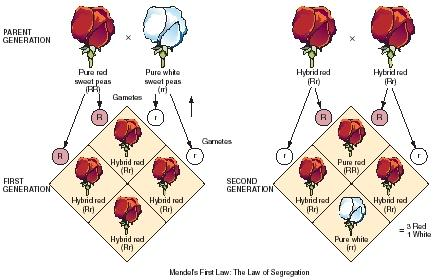
\includegraphics[scale=.75]{./diagrams/mendel.jpg}
\end{figure}
\end{frame}

\begin{frame}
  \frametitle{Exercises}
{\ubung} Your friend tosses two coins. You don't see the
coins, but your friend tells you that at least one of them landed
heads. What is the probability that they both landed heads?

{\ubung} Alice and Branden have brown eyes. Their son Joel has blue
eyes. What is the probability that their next child will have blue
eyes as well?

{\ubung} In a sample of 207 adults, 43 are smokers. What
is the probability of choosing a person at random who is a smoker?
\end{frame}

\begin{frame}
  \frametitle{Exercises}
{\ubung} A game show host asks you a multiple choice
question with four answers A, B, C, and D. If you make a random guess,
what is your probability of getting the correct answer?

{\ubung} In a country far away, all parents want to have
girls. The probability of having a girl is 50\%. All parents have boys
until they have a girl. What would you expect to be the proportion of
girls in that country?

{\ubung} The government found out that 102 out of 810
luggage scales at the airport are defective. If you choose 2 luggage
scales at random \emph{with replacement}, what is the probability that
they are both defective? If you choose 2 luggage scales at random
\emph{without replacement}, what is the probability that they are both
defective?
\end{frame}

\begin{frame}
  \frametitle{Tree Diagrams I}
{\ubung} The probability that BCIT hires a person on a
particular weekday is the same as any other weekday. What is the
probability that two randomly selected employees were both hired on a
Monday? What is the probability that two randomly selected employees
were both hired on the same weekday?

{\ubung} In a group of people, 492 would choose a window
seat on an airplane, 8 would choose a middle seat, and 306 would
choose an aisle seat. What is the probability of randomly choosing a
person who would not choose a middle seat? What is the probability of
randomly choosing two people who would not choose a middle seat? What
is the probability of randomly choosing twenty-five people who would
not choose a middle seat?
\end{frame}

\begin{frame}
  \frametitle{Tree Diagrams II}
{\ubung} What is the probability of rolling a sum of 9 on
two dice rolls?

{\ubung} What is the probability of having two girls and
three boys when there are five children and the probability of having
a boy is 50\%?
\end{frame}

\begin{frame}
  \frametitle{Tree Diagrams}
You can use independence and mutual exclusion to draw tree diagrams.
\begin{figure}[h]
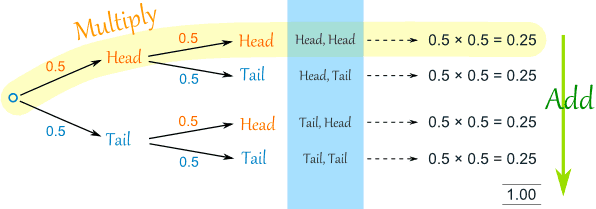
\includegraphics[scale=.5]{./diagrams/tree.png}
\end{figure}
\end{frame}

\begin{frame}
  \frametitle{Exercise Tree Diagram}
{\ubung} You have two coaches, Sam and Alex. When Sam
coaches the team, your proability of being the goalkeeper is 50\%. When Alex
coaches the team, your proability of being the goalkeeper is 30\%. The
probability that Sam (rather than Alex) will coach your team today is
60\%. What is the probability that you will be goalkeeper?
\end{frame}

\newcommand{\sam}{.65}

\begin{frame}
  \frametitle{Sam and Alex I}
\begin{figure}[h]
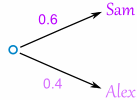
\includegraphics[scale=\sam]{./diagrams/sam1.png}
\end{figure}
\end{frame}

\begin{frame}
  \frametitle{Sam and Alex II}
\begin{figure}[h]
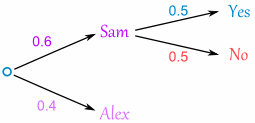
\includegraphics[scale=\sam]{./diagrams/sam2.png}
\end{figure}
\end{frame}

\begin{frame}
  \frametitle{Sam and Alex III}
\begin{figure}[h]
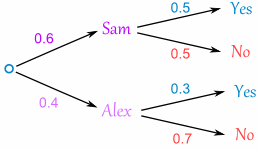
\includegraphics[scale=\sam]{./diagrams/sam3.png}
\end{figure}
\end{frame}

\begin{frame}
  \frametitle{Sam and Alex IV}
\begin{figure}[h]
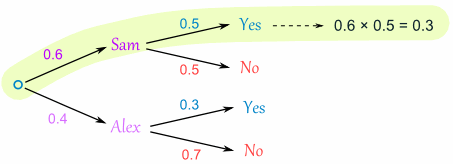
\includegraphics[scale=\sam]{./diagrams/sam4.png}
\end{figure}
\end{frame}

\begin{frame}
  \frametitle{Sam and Alex V}
\begin{figure}[h]
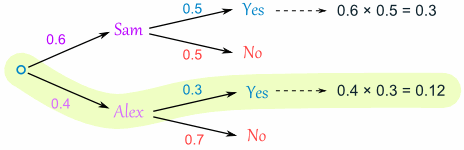
\includegraphics[scale=\sam]{./diagrams/sam5.png}
\end{figure}
\end{frame}

\begin{frame}
  \frametitle{Sam and Alex VI}
\begin{figure}[h]
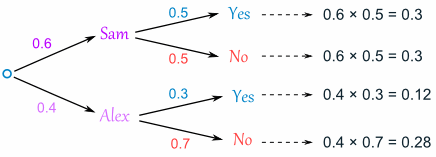
\includegraphics[scale=\sam]{./diagrams/sam6.png}
\end{figure}
\end{frame}

\begin{frame}
  \frametitle{How to Solve Probability Problems}
In summary, here are some strategies to solve probability problems.
\begin{enumerate}
\item Count simple events. If the simple events are all equally
  probable, then the probability of event $A$ is the number of simple
  events in $A$ divided by the total number of simple events, so
  $P(A)=\#A/\#\Omega$.
\item Make sure to watch for independence and mutual exclusion.
  Whenever events are independent or mutually exclusive (disjoint),
  you can use $P(A\cap{}B)=P(A)P(B)$ or $P(A\cup{}B)=P(A)+P(B)$,
  respectively.
\item If events are not mutually exclusive, you can use the
  addition rule $P(A\cup{}B)=P(A)+P(B)-P(A\cap{}B)$.
\item If events are not independent, you can use conditional
  probabilities in $P(A\cap{}B)=P(A)P(B|A)$.
\item If you are dealing with events that are independent and
  mutually exclusive, it is often useful to draw a tree diagram.
\end{enumerate}
\end{frame}

\begin{frame}
  \frametitle{xkcd on Bayes' Formula}
\begin{figure}[h]
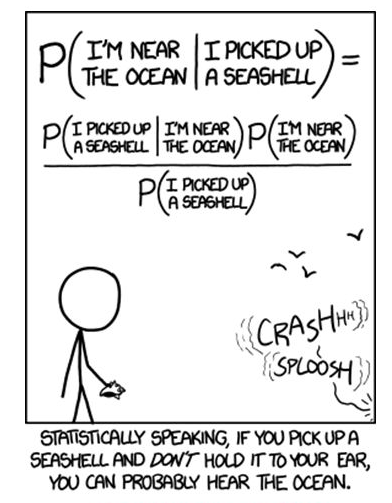
\includegraphics[scale=.5]{./diagrams/xkcd_bayes1.png}
\end{figure}
\end{frame}

% \begin{frame}
%   \frametitle{Two Examples}
% Here are two of my own examples.
% http://psycnet.apa.org/record/1975-11611-001 and
% https://derstandard.at/2000076668166/Mythos-oder-wahr-Durch-Abschrecken-lassen-sich-Eier-besser-schaelen

% For the second one: What is the probability that an egg is fresh when
% it is a crater egg? For the first one: What is the probability of
% being attractive when you are accepted?
% \end{frame}

\begin{frame}
  \frametitle{Conditional Probability}
Let's remember what conditional probability means.
% \begin{equation}
%   \label{eq:ohyeweeb}
%   P(B|A)=\frac{P(B\cap{}A}{P(A)}
% \end{equation}
\begin{figure}[h]
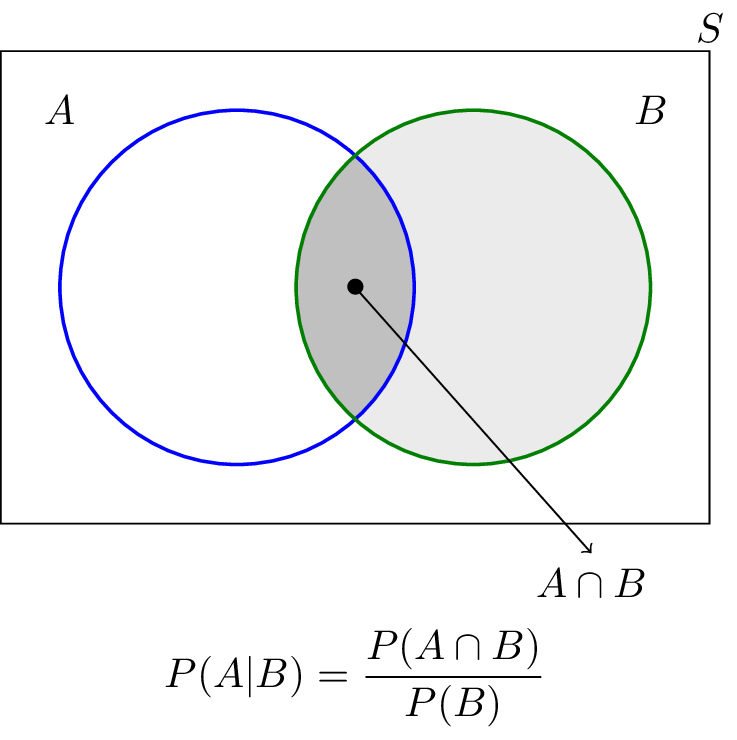
\includegraphics[scale=.25]{./diagrams/conditional_b.png}
\end{figure}
\end{frame}

\begin{frame}
  \frametitle{Multiplication Rule}
  Remember the thief who wants to crack the four-digit PIN of a bank
  card. Let $A$ be the event that she successfully cracks the PIN. If
  $A_{1}$ is the event that she succeeds on her first attempt (and so
  on for $A_{2}$ and $A_{3}$), then
\begin{equation}
  \label{eq:ragheidu}
  P(A)=P(A_{1}\cup{}A_{2}\cup{}A_{3})=P(A_{1})+P(A_{2})+P(A_{3})=0.003
\end{equation}
because $A_{1},A_{2},A_{3}$ are disjoint. We are assuming that her
attempts happen \alert{without replacement}. Therefore,
$A_{1},A_{2},A_{3}$ are not independent, and the correct application of
the multiplication rule is
\begin{equation}
  \label{eq:mohghunu}
  P(A)=1-P(\urcorner{}A)=\notag
\end{equation}
\begin{equation}
  \label{eq:yoobaegh}
  1-P(\urcorner{}A_{1})\cdot{}P(\urcorner{}A_{2}|\urcorner{}A_{1})\cdot{}P(\urcorner{}A_{3}|\urcorner{}A_{1}\cap{}\urcorner{}A_{2})=0.003
\end{equation}
\end{frame}

\begin{frame}
  \frametitle{Law of Total Probability}
It is often easier to calculate conditional probabilities than
unconditional probabilities. To express one by the other use the
\alert{law of total probability},
\begin{equation}
  \label{eq:aefengah}
  P(A)=P(A|B)P(B)+P(A|\urcorner{}B)P(\urcorner{}B)
\end{equation}
This formula also applies when you split up $B$ into three or more
disjoint subsets that exhaust $B$. It follows from set theory.

\bigskip

\textbf{Example: }Suppose that two factories supply light bulbs to the
market. Factory X's bulbs work for over 5000 hours in 99\% of cases,
whereas factory Y's bulbs work for over 5000 hours in 95\% of cases.
It is known that factory X supplies 60\% of the total bulbs available.
What is the chance that a purchased bulb will work for longer than
5000 hours?
% Now we should be able to answer the question from last week: How many
% four digit numbers are there with no repeating digits?
\end{frame}

\begin{frame}
  \frametitle{Law of Total Probability}
\textbf{Example: }Suppose that two factories supply light bulbs to the
market. Factory X's bulbs work for over 5000 hours in 99\% of cases,
whereas factory Y's bulbs work for over 5000 hours in 95\% of cases.
It is known that factory X supplies 60\% of the total bulbs available.
What is the chance that a purchased bulb will work for longer than
5000 hours?

\bigskip

Let $X$ be the event that the light bulb is from factory X. Let $F$ be
the event that the bulb will work for longer than
5000 hours. Then
\begin{equation}
  \label{eq:uwahiamo}
  P(F)=P(F|X)P(X)+P(F|\urcorner{}X)P(\urcorner{}X)=\notag
\end{equation}
\begin{equation}
  \label{eq:siecafoo}
  0.99\cdot{}0.60+0.95\cdot{}0.40=0.974
\end{equation}
\end{frame}

\begin{frame}
  \frametitle{Law of Total Probability Exercises I}
What is the probability that the second card in a conventional
deck of cards is an ace?
\end{frame}

\begin{frame}
  \frametitle{Law of Total Probability Exercises II}
Suppose we have two hats: one has 4 red balls and 7 green balls,
the other has 11 red and 5 green. We toss an unfair coin (60/40 for
heads), if heads, pick a random ball from the first hat, if tails from
the second. What is the probability of getting a red ball?
\end{frame}

\begin{frame}
  \frametitle{Law of Total Probability Exercises III}
You have three bags that each contain 100 marbles:
\begin{itemize}
\item Bag 1 has 75 red and 25 blue marbles
\item Bag 2 has 60 red and 40 blue marbles
\item Bag 3 has 45 red and 55 blue marbles
\end{itemize}
I choose one of the bags at random and then pick a marble from the
chosen bag, also at random. What is the probability that the chosen
marble is red?
\end{frame}

\begin{frame}
  \frametitle{Some Interesting Cases}
  A group of police officers have breathalyzers displaying false
  drunkenness in 5\% of the cases in which the driver is sober.
  However, the breathalyzers never fail to detect a truly drunk
  person. One in a thousand drivers is driving drunk. Suppose the
  police officers then stop a driver at random, and force the driver
  to take a breathalyzer test. It indicates that the driver is drunk.
  We assume you don't know anything else about him or her. How high is
  the probability he or she really is drunk?
\end{frame}

\begin{frame}
  \frametitle{Some Interesting Cases}
  A room is full of engineers and lawyers (most of them are lawyers,
  90\%). The probability that an engineer enjoyed physics in school is
  80\%. The probability that a lawyer enjoyed physics in school is
  30\%. You ask someone in the room whether they enjoyed physics, and
  the answer is yes. Should you bet that this person is a lawyer, or
  should you bet that she is an engineer?
\end{frame}

\begin{frame}
  \frametitle{Some Interesting Cases}
You have a million food items, of which 1 in 1000 is contaminated. You
have a contamination test with a 2\% false positive rate and a 0.5\%
false negative rate. A food item tests positive for contamination.
What is the probability that it is contaminated?
\end{frame}

\begin{frame}
  \frametitle{Some Interesting Cases}
  In a city of 1 million inhabitants let there be 100 terrorists and
  999,900 non-terrorists. To simplify the example, it is assumed that
  all people present in the city are inhabitants. Thus, the base rate
  probability of a randomly selected inhabitant of the city being a
  terrorist is 0.0001, and the base rate probability of that same
  inhabitant being a non-terrorist is 0.9999. In an attempt to catch
  the terrorists, the city installs an alarm system with a
  surveillance camera and automatic facial recognition software.

The software has two failure rates of 1\%:
\begin{itemize}
\item The false negative rate: If the camera scans a terrorist, a bell
  will ring 99\% of the time, and it will fail to ring 1\% of the
  time.
\item The false positive rate: If the camera scans a non-terrorist, a
  bell will not ring 99\% of the time, but it will ring 1\% of the
  time.
\end{itemize}

Suppose now that an inhabitant triggers the alarm. What is the chance
that the person is a terrorist?
\end{frame}

\begin{frame}
  \frametitle{Bayes' Formula}
Consider the definition of conditional probability,
\begin{equation}
  \label{eq:ohyeweeb}
  P(B|A)=\frac{P(B\cap{}A)}{P(A)}
\end{equation}
Now notice that $P(B\cap{}A)=P(A\cap{}B)=P(B)P(A|B)$. That means that
\begin{equation}
  \label{eq:maifiepu}
  P(B|A)=\frac{P(B)P(A|B)}{P(A)}
\end{equation}
By the law of total probability we can replace the denominator to give
us \alert{Bayes' Formula}
\begin{equation}
  \label{eq:ohrughai}
  P(B|A)=\frac{P(B)P(A|B)}{P(A|B)P(B)+P(A|\urcorner{}B)P(\urcorner{}B)}
\end{equation}
\end{frame}

\begin{frame}
  \frametitle{Base Rate Fallacy Diagram}
\begin{figure}[h]
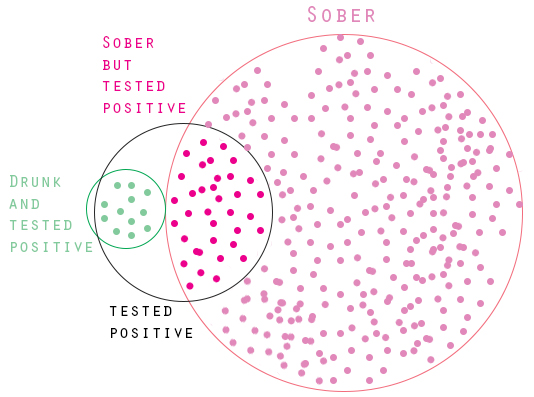
\includegraphics[scale=.4]{./diagrams/Detect-drunk-driving.jpg}
\end{figure}
\end{frame}

\begin{frame}
  \frametitle{Base Rate Fallacy Example}
  Let 100 out of 100,000 people have a disease. The test for this
  disease has a 5\% \alert{false positive} rate and a 5\% \alert{false
    negative} rate. If you test positive for this disease, what is
  your probability of actually having the disease. Consider the
  following \alert{contingency table} and then apply Bayes'
  formula.
\begin{figure}[h]
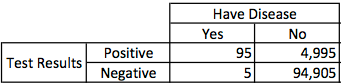
\includegraphics[scale=.7]{./diagrams/baserate3.png}
\end{figure}
\end{frame}

\begin{frame}
  \frametitle{Contingency Tables}
\begin{figure}[h]
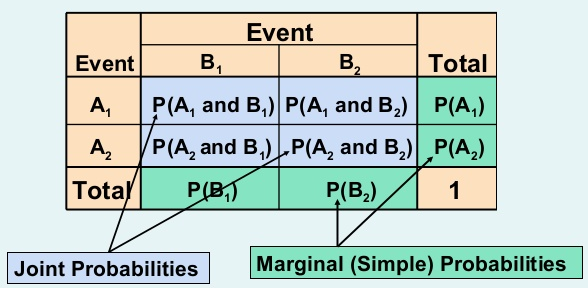
\includegraphics[scale=.5]{./diagrams/contingency1.png}
\end{figure}
\end{frame}

\begin{frame}
  \frametitle{Prison and Plea}
Here is a contingency table:
\begin{tabular}{|l|c|c|}\hline
  & Guilty Plea & Plea of Not Guilty \\ \hline
  Sentenced to Prison & 392 & 58 \\ \hline
  Not Sentenced to Prison & 564 & 14 \\ \hline
\end{tabular}
\end{frame}

\begin{frame}
  \frametitle{Prison and Plea}
Answer the following questions:
\begin{enumerate}
\item Find the probability of a randomly selected subject being
  sentenced to prison.
\item Find the probability of being sentenced to prison, given
  that the subject entered a plea of guilty.
\item Find the probability of being sentenced to prison, given
  that the subject entered a plea of not guilty.
\item Find the probability of a randomly selected subject being
  sentenced to prison or entering a plea of guilty.
\end{enumerate}
\end{frame}

\begin{frame}
  \frametitle{Prison and Plea}
Answer the following questions:
\begin{enumerate}
\setcounter{enumi}{4}
\item If two subjects are randomly selected, find the probability
  that they were both sentenced to prison.
\item If two subjects are randomly selected, find the probability
  that they both entered pleas of not guilty.
\item Find the probability of a randomly selected subject being
  entering a plea of not guilty or not being sentenced to prison.
\item Find the probability of a randomly selected subject being
  sentenced to prison and entering a plea of guilty.
\item Find the probability of a randomly selected subject not being
  sentenced to prison and not entering a plea of guilty.
\end{enumerate}
\end{frame}

\begin{frame}
  \frametitle{Exercises I}
% J.V. Uspensky, Introduction to Mathematical Probability, p40
Three urns contain respectively 1 white and 2 black balls; 3 white and
1 black ball; 2 white and 3 black balls. One ball is taken from each
urn. What is the probability that among the balls drawn there are 2
white and 1 black?
\end{frame}

\begin{frame}
  \frametitle{Exercises I}
% J.V. Uspensky, Introduction to Mathematical Probability, p40
Three urns contain respectively 1 white and 2 black balls; 3 white and
1 black ball; 2 white and 3 black balls. One ball is taken from each
urn. What is the probability that among the balls drawn there are 2
white and 1 black? Answer: $23/60$
\end{frame}

\begin{frame}
  \frametitle{Exercises II}
% Devore and Peck, Statistics, p247
A student has a box containing 25 computer disks, of which 15 are
blank and 10 are not. She randomly selects disks one by one and
examines each one, terminating the process only when she finds a blank
disk. What is the probability that she must examine at least two disks?
\end{frame}

\begin{frame}
  \frametitle{Exercises II}
% Devore and Peck, Statistics, p247
A student has a box containing 25 computer disks, of which 15 are
blank and 10 are not. She randomly selects disks one by one and
examines each one, terminating the process only when she finds a blank
disk. What is the probability that she must examine at least two
disks? Answer: 40\%
\end{frame}

\begin{frame}
  \frametitle{Exercises III}
% Devore and Peck, Statistics, p247
There are five faculty members in a certain academic department. These
individuals have 3, 6, 7, 10, and 14 years of teaching experience,
respectively. Two of these individuals are randomly selected to serve
on a committee. What is the probability that they have at least 15
years of teaching experience?
\end{frame}

\begin{frame}
  \frametitle{Exercises III}
% Devore and Peck, Statistics, p247
There are five faculty members in a certain academic department. These
individuals have 3, 6, 7, 10, and 14 years of teaching experience,
respectively. Two of these individuals are randomly selected to serve
on a committee. What is the probability that they have at least 15
years of teaching experience? Answer: 60\%
\end{frame}

\begin{frame}
  \frametitle{Exercises IV}
% Devore and Peck, Statistics, p249
Suppose three cards are selected from a well-mixed deck without
replacement. 
\begin{enumerate}
\item<1-> What is the probability that all three are hearts?
\item<2-> What is the probability that all three are from the same
  suit?
\item<3-> If five cards are dealt from a randomized deck, determine
  the probability that they are all hearts.
\end{enumerate}
\end{frame}

\begin{frame}
  \frametitle{Exercises IV}
% Devore and Peck, Statistics, p249
Suppose three cards are selected from a well-mixed deck without
replacement. 
\begin{enumerate}
\item What is the probability that all three are hearts? Answer: $1.29$\%
\item What is the probability that all three are from the same
  suit? Answer: $5.18$\%
\item If five cards are dealt from a randomized deck, determine
  the probability that they are all hearts. Answer: $0.0495$\%
\end{enumerate}
\end{frame}

\begin{frame}
  \frametitle{Exercises V}
% Devore and Peck, Statistics, p250
  A tennis coach has brought out 12 tubes of Penn balls and 8 tubes of
  Wilson balls for his class. If 5 tubes are randomly selected, what
  is the probability that all 5 are of the same brand?
\end{frame}

\begin{frame}
  \frametitle{Exercises V}
% Devore and Peck, Statistics, p250
  A tennis coach has brought out 12 tubes of Penn balls and 8 tubes of
  Wilson balls for his class. If 5 tubes are randomly selected, what
  is the probability that all 5 are of the same brand? Answer: $5.47$\%
\end{frame}

\begin{frame}
  \frametitle{Exercises VI}
\begin{figure}[h]
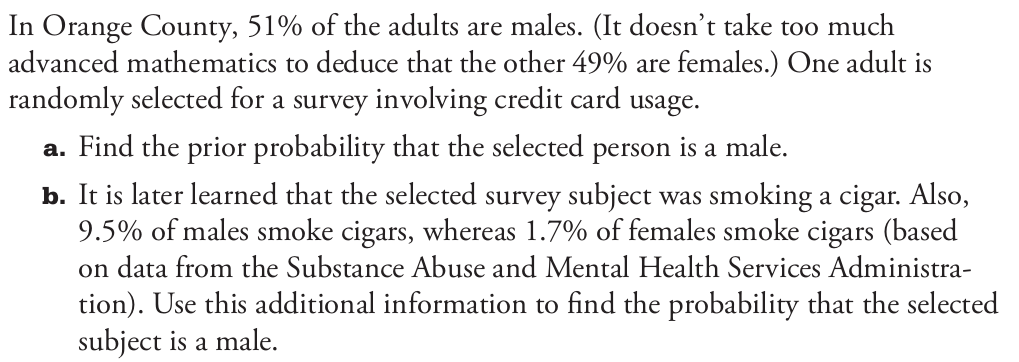
\includegraphics[scale=.32]{./diagrams/triola_bayes1.png}
\end{figure}
\end{frame}

\begin{frame}
  \frametitle{Exercises VI}
\begin{figure}[h]
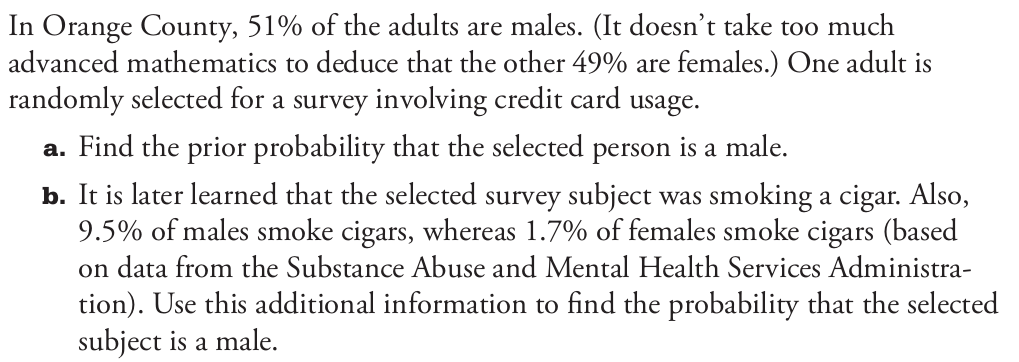
\includegraphics[scale=.32]{./diagrams/triola_bayes1.png}
\end{figure}
Answer: (a.) $51$\% (b.) $85.3$\%
\end{frame}

\begin{frame}
  \frametitle{Exercises VII}
\begin{figure}[h]
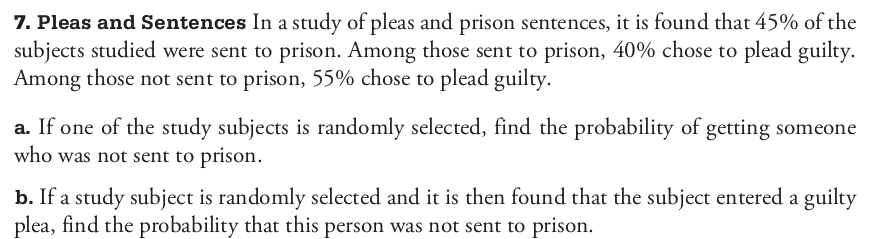
\includegraphics[scale=.36]{./diagrams/triola_bayes2.png}
\end{figure}
\end{frame}

\begin{frame}
  \frametitle{Exercises VII}
\begin{figure}[h]
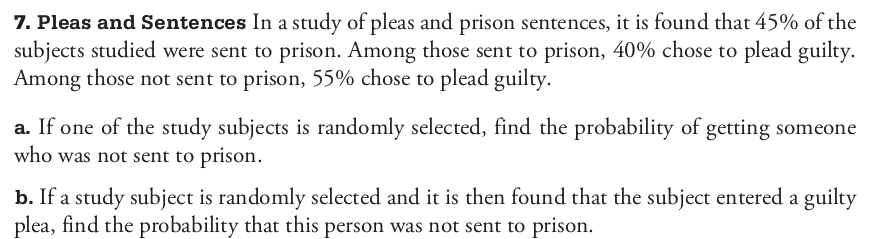
\includegraphics[scale=.36]{./diagrams/triola_bayes2.png}
\end{figure}
Answer: (a.) $55$\% (b.) $62.7$\%
\end{frame}

\begin{frame}
  \frametitle{Exercises VIII}
\begin{figure}[h]
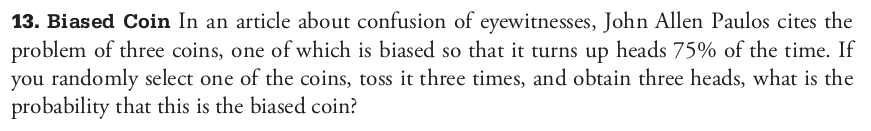
\includegraphics[scale=.36]{./diagrams/triola_bayes3.png}
\end{figure}
\end{frame}

\begin{frame}
  \frametitle{Exercises VIII}
\begin{figure}[h]
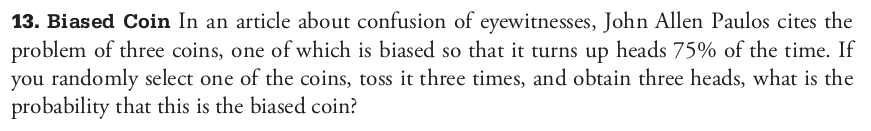
\includegraphics[scale=.36]{./diagrams/triola_bayes3.png}
\end{figure}
Answer: $62.8$\%
\end{frame}

\begin{frame}
  \frametitle{Probability Distributions: Concepts}
Here are some definitions.
\begin{description}
\item[random variable] A random variable is a variable (typically
  represented by $X$) that has a single numerical value, determined by
  chance, for each outcome of a procedure.
\item[probability distribution] A probability distribution is a
  description that gives the probability for each value of the random
  variable. It is often expressed in the format of a table, formula,
  or graph.
\end{description}
\end{frame}

\begin{frame}
  \frametitle{Probability Distributions: Discrete and Continuous}
\begin{description}
\item[discrete random variable] A \alert{discrete} random variable has
  a collection of values that is finite or countable.
\item[continuous random variable] A \alert{continuous} random variable has
  infinitely many values, and the collection of values is not
  countable.
\item[countability] This is best explained by example: the integers
  are countable, but the real numbers are not.
\end{description}
\end{frame}

\begin{frame}
  \frametitle{Discrete Probability Distributions}
  If there are a finite number of outcomes $X=a_{k}$ for
  $k=1,\ldots,n$, we can list the values of $P(X=a_{k})$ in a table. 

\bigskip

\beispiel{Coin Toss}\label{ex:ootiteij} let $X=1$ for heads and $X=0$
for tails. Then 

\bigskip

\begin{tabular}{|l|l|}\hline
  Event & Probability \\ \hline
  $X=1$ or $H$ & 0.50 \\ \hline
  $X=0$ or $T$ & 0.50 \\ \hline
\end{tabular}

\bigskip

When all the probabilities are equal, we call the probability
distribution a \alert{uniform distribution}.
\end{frame}

\begin{frame}
  \frametitle{Non-Uniform Discrete Probability Distributions}
  Some distribution probability distributions are not uniform.

\bigskip

  \beispiel{Number of Male Children}\label{ex:shaisail} Consider the
  two-child family. If $X$ is the random variable corresponding to the
  number of boys in the family, then the probability distribution
  table looks as follows (assuming that the probability distribution
  for one child is uniform).
\end{frame}

\begin{frame}
  \frametitle{Discrete Probability Distribution Graphs I}
\begin{tabular}{|l|l|}\hline
  Event & Probability \\ \hline
  $X=2$ or two boys & 0.25 \\ \hline
  $X=1$ or one boy, one girl & 0.50 \\ \hline
  $X=0$ or two girls & 0.25 \\ \hline
\end{tabular}

\bigskip

\begin{figure}[h]
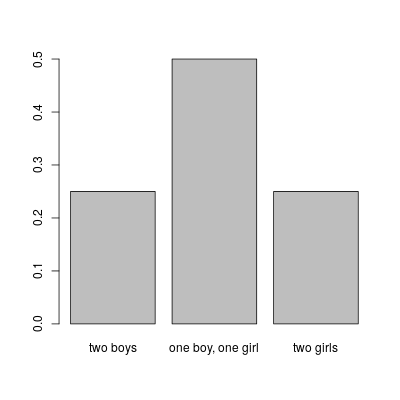
\includegraphics[scale=.45]{./diagrams/boys.png}
\end{figure}
\end{frame}

\begin{frame}
  \frametitle{Discrete Probability Distribution Graphs II}
  \beispiel{Immigrant Languages}\label{ex:ahchoiyu} Here is the
  probability distribution for a randomly selected ``Vancouverite''
  (Greater Vancouver) to speak a certain immigrant language at home.

\vspace{-.5in}

\begin{figure}[h]
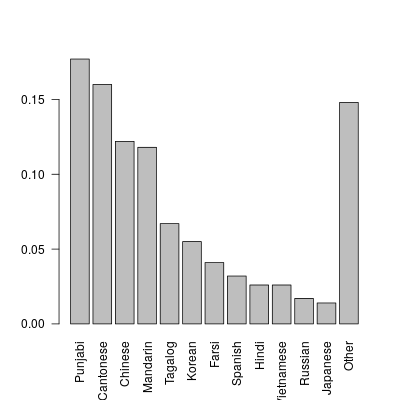
\includegraphics[scale=.5]{./diagrams/vanlang.png}
\end{figure}
\end{frame}

\begin{frame}
  \frametitle{Mean and Variance Formulas}
There is a sense in which a probability distribution together with its
associated random variable correspond to a population and the property
which the random variable picks out. In this spirit, let us define a
mean and a variance for a probability distribution.
\begin{equation}
  \label{eq:noohahfa}
  \mu=\sum{}X\cdot{}P(X)
\end{equation}
\begin{equation}
  \label{eq:axiengeb}
  \sigma^{2}=\sum(X-\mu)^{2}\cdot{}P(X)
\end{equation}
\begin{equation}
  \label{eq:teeneilu}
  \sigma^{2}=\sum(X^{2}\cdot{}P(X))-\mu^{2}
\end{equation}
\begin{equation}
  \label{eq:iifiekai}
  \sigma=\sqrt{\sum(X^{2}\cdot{}P(X))-\mu^{2}}
\end{equation}
\end{frame}

\begin{frame}
  \frametitle{Die Roll Example}
\beispiel{Fair Die Roll}\label{ex:reinooth} Think of rolling a fair die
many times. The probability distribution is uniform. The mean is
\begin{equation}
  \label{eq:isiamaih}
   \mu=\sum{}X\cdot{}P(X)=1\cdot{}\frac{1}{6}+2\cdot{}\frac{1}{6}+3\cdot{}\frac{1}{6}+4\cdot{}\frac{1}{6}+5\cdot{}\frac{1}{6}+6\cdot{}\frac{1}{6}=3.5\notag
\end{equation}
We also call this number the \alert{expectation} $EX$ of the random
variable $X$. Although you would never expect a die roll to result in
``3.5,'' you would expect the mean of many die rolls to be close to
this number. The expected number of boys for one birth is $EX=0.5$.
\end{frame}

\begin{frame}
  \frametitle{The Binomial Probability Distribution}
A \alert{binomial probability distribution} results from a procedure
that meets the following requirements.
\begin{enumerate}
\item The procedure has a fixed number of trials.
\item The trials must be independent.
\item The outcomes of a trial are binary, i.e.\ there are only two
  possible outcomes.
\item The probability of the two outcomes remains constant.
\end{enumerate}
The number of trials is usually labeled $n$, the two outcomes are
called \alert{success} and \alert{failure}, and their probabilities on
one trial are $p$ and $1-p$. The random variable keeps track of the
number of successes. If, for example, there are 10 trials, then
$P(X=4)$ is the probability of 4 successes out of 10. The number of
successes is often labeled $x$, and we are usually interested in
$P(X=x)$.
\end{frame}

\begin{frame}
  \frametitle{Calvin on the Binomial Distribution}
\begin{figure}[h]
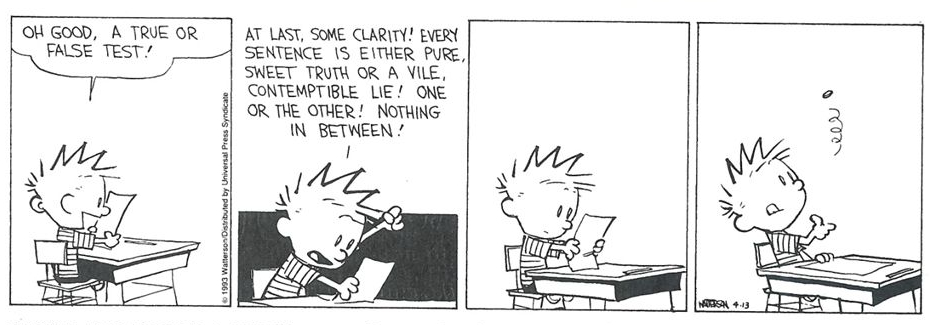
\includegraphics[scale=.43]{./diagrams/calvin_hobbes_binomial_edited.jpg}
\end{figure}
\end{frame}

\begin{frame}
  \frametitle{The Binomial Probability Formula}
If $n,p,x$ are as described on the previous slide, then
\begin{equation}
  \label{eq:pheehael}
  % P(X=x)={n\choose{}x}\cdot{}p^{x}\cdot(1-p)^{n-x}
  P(X=x)=\binom{n}{x}\cdot{}p^{x}\cdot(1-p)^{n-x}
\end{equation}
\end{frame}

\begin{frame}
  \frametitle{Exercises for the Binomial Distribution I}
  {\ubung} If you randomly guess on a multiple choice test with four
  possible answers, what is your probability of getting strictly more than 50\%
  of questions right when there are six questions?
\end{frame}

\begin{frame}
  \frametitle{Exercises for the Binomial Distribution II}
  {\ubung} The incidence of blue eyes in the population is 12\%. In a room
  with 20 randomly selected people, what is the probability of having
  three or more people with blue eyes? What is the probability of
  having strictly fewer than five people with blue eyes? 
  \begin{quote}
    Strictly speaking, the binomial probabilities are only approximate
    because the selection happens without replacement. If the
    population is large from which the sample is drawn, then you are
    allowed to ignore this.
  \end{quote}
\end{frame}

\begin{frame}
  \frametitle{Exercises for the Binomial Distribution III}
  {\ubung} Here is the distribution of blood types in Canada.

\bigskip

  \begin{tabular}{|l|r|r|r|r|}\hline
         & O     & A     & B     & AB    \\ \hline
Positive & 0.390 & 0.360 & 0.076 & 0.025 \\ \hline
Negative & 0.070 & 0.060 & 0.014 & 0.005 \\ \hline
  \end{tabular}

\bigskip

(a) What is the probability of being rhesus factor positive for
someone of blood type ``A''?

\medskip

(b) If you meet four randomly selected Canadians, what is the
probability that two of them are ``O'' positive?

\medskip

(c) In a room with twelve randomly selected Canadians, what is the
probability that there are strictly fewer than three people with
blood type ``B''?
\end{frame}

\begin{frame}
  \frametitle{Exercises for the Binomial Distribution IV}
  {\ubung} 80.5\% of US flights arrive on time. For twelve randomly
  selected flights, what is the probability that exactly ten of them
  are on time? What is the probability that between two and four of
  them are not on time?
\end{frame}

\begin{frame}
  \frametitle{Mean and Variance for the Binomial Distribution}
There are formulas for the mean and variance of the binomial
distribution. Especially the formula for the mean makes immediate
sense:
\begin{block}{Formulas}
  \begin{tabular}{llcr}
  mean& $\mu$&$=$&$np$ \\ 
  variance& $\sigma^{2}$&$=$&$npq$ \\
  standard deviation& $\sigma$&$=$&$\sqrt{npq}$
  \end{tabular}
\end{block}
It is a useful rule of thumb to remember that it is unlikely ($<5\%$)
that $x$ is outside of the interval from $\mu-2\sigma$ to
$\mu+2\sigma$.
\end{frame}

\begin{frame}
  \frametitle{Exercises for the Binomial Distribution V}
  {\ubung} What is the rule-of-thumb 95\% interval for the following
  binomial procedures:
  \begin{enumerate}
\item<1-> flipping a fair coin 15 times
\item<2-> answering 60 multiple choice questions with four possible
  answers for each question, where the probability of getting the right answer is 80\%
\item<3-> randomly answering 60 multiple choice questions with four
  possible answers for each question
\item<4-> The number of ``O'' positive blood types in a crowd of 100 Canadians.
  \end{enumerate}
\end{frame}

\begin{frame}
  \frametitle{Word Problems}
  {\ubung} Based on observed males using public restrooms, 85\% of
  adult males wash their hands in a public restroom (based on data
  from the American Society for Microbiology and the American Cleaning
  Institute). In a survey of 523 adult males, 518 reported that they
  wash their hands in a public restroom. Assuming that the 85\%
  observed rate is correct, find the probability that among 523
  randomly selected adult males, 518 or more wash their hands in a
  public restroom. What do you conclude?
\end{frame}

\begin{frame}
  \frametitle{Word Problems}
  {\ubung} In a survey of 1002 people, 701 said that they voted in a
  recent presidential election (based on data from ICR Research
  Group). Voting records show that 61\% of eligible voters actually
  did vote. Given that 61\% of eligible voters actually did vote, find
  the probability that among 1002 randomly selected eligible voters,
  at least 701 actually did vote. What does the result suggest?
\end{frame}

\begin{frame}
  \frametitle{Word Problems}
  {\ubung} In a study of 420,095 cell phone users in Denmark, it was
  found that 135 developed cancer of the brain or nervous system.
  Assuming that the use of cell phones has no effect on developing
  such cancers, there is a 0.000340 probability of a person developing
  cancer of the brain or nervous system. We therefore expect about 143
  cases of such cancers in a group of 420,095 randomly selected
  people. Estimate the probability of 135 or fewer cases of such
  cancers in a group of 420,095 people. What do these results suggest
  about media reports that cell phones cause cancer of the brain or
  nervous system?
\end{frame}

\begin{frame}
  \frametitle{Word Problems}
  {\ubung} Based on a recent Harris Interactive survey, 20\% of adults
  in the United States smoke. In a survey of 50 statistics students,
  it is found that six of them smoke. Find the probability that should
  be used for determining whether the 20\% rate is correct for
  statistics students. What do you conclude?
\end{frame}

\begin{frame}
  \frametitle{Word Problems}
  {\ubung} Online TV In a Comcast survey of 1000 adults, 17\% said
  that they watch prime-time TV online. If we assume that 20\% of
  adults watch prime-time TV online, find the probability that should
  be used to determine whether the 20\% rate is correct or whether it
  should be lower than 20\%? What do you conclude?
\end{frame}

\begin{frame}
  \frametitle{Word Problems}
  {\ubung} Internet Access Of U.S. households, 67\% have Internet
  access (based on data from the Census Bureau). In a random sample of
  250 households, 70\% are found to have Internet access. Find the
  probability that should be used to determine whether the 67\% rate
  is too low. What do you conclude?
\end{frame}

\begin{frame}
  \frametitle{End of Lesson}
Next Lesson: Central Limit Theorem
\end{frame}

\end{document}
